\section{Propuesta de solución}

La empresa requirió que las soluciones de la cinemática inversa se guardaran en un archivo, que posteriormente sea reproducido y enviado desde el software SettDev al PLC-Kaab. De este modo, la propuesta de solución se dividió en dos fases. La Figura \ref{fig:fasecaptura} muestra la primera fase, la de captura de datos. En la etapa de Sensado, el sensor MPU-6050 mide la orientación del sensor, y envía los ángulos de inclinación $S(\theta_x, \theta_y, \theta_z)$ calculados en los 3 ejes a la Raspberry Pi. Estos valores son la entrada de la etapa de Localización, en la cual se determina la posición $(x, y, z)$ en el espacio de la muñeca respecto al hombro (quien tiene la posición $(0, 0, 0)$), que será la que deberá alcanzar el efector final. Estas coordenadas sirven como entrada a la red neuro-difusa en la etapa de Procesamiento, donde, de acuerdo con la longitud de las articulaciones $(L_1, L_2)$ especificada mediante una interfaz, se calculan los ángulos $(\alpha_1, \alpha_2, \alpha_3)$ que resuelven la cinemática inversa para alcanzar la posición $(x, y, z)$ previamente calculada. Estos ángulos se aplican al movimiento de un modelo de brazo robótico en 2D en la interfaz gráfica antes mencionada en la etapa de Visualización, en la que se puede simular el comportamiento que tendría el brazo robótico al aplicar dichos ángulos, así como al movimiento de un modelo de brazo robótico en 3D en la etapa de Referencia. Finalmente, los ángulos $(\alpha_1, \alpha_2, \alpha_3)$ son almacenados en un archivo con extensión .bin.

\begin{figure}[htb]
	\centering
	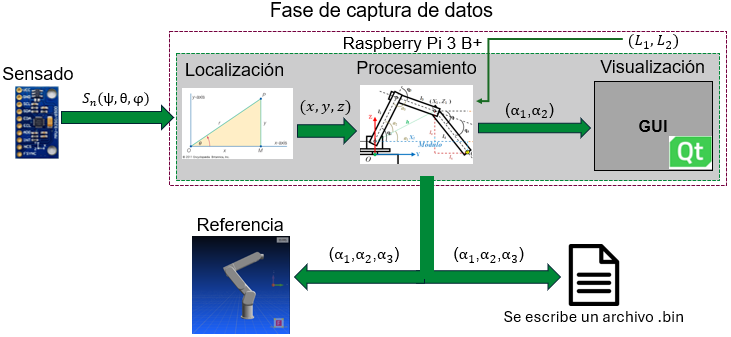
\includegraphics[scale=0.85]{fasecaptura.png}
	\caption{Fase de captura de datos}
	\label{fig:fasecaptura}
\end{figure}

\newpage
La Figura \ref{fig:faseejecucion} muestra la segunda fase, la de ejecución. El archivo con extensión .bin previamente guardado es leído y transmitido por el software SettDev hacia el PLC-Kaab, quien interpreta los ángulos recibidos y los modula en ancho de pulso para controlar la posición de los servomotores posicionales.

\begin{figure}[htb]
	\centering
	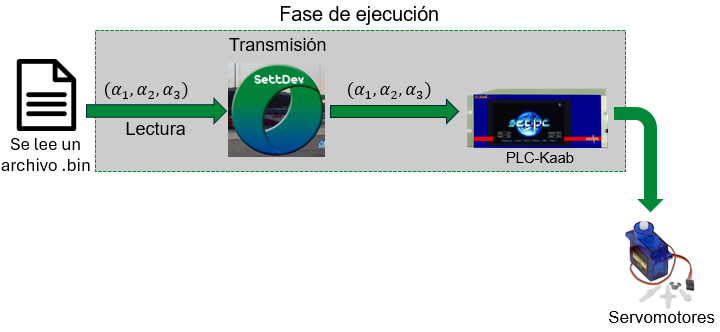
\includegraphics[scale=0.85]{faseejecucion.png}
	\caption{Fase de ejecución}
	\label{fig:faseejecucion}
\end{figure}